\DiaryEntry{Projection onto a Plane}{2017-10-04}{Maths}

Consider the following optimization problem

\[
\hat{\mathbf{x}} = \arg \min || \mathbf{y} - \mathbf{Ax} ||^2
\]

where \(\mathbf{x,\hat{x}, y}\) are \(n\)-element vectors and \(\mathbf{A}\) is an \(n \times m\) matrix. We can interpret the problem that the columns of \(\mathbf{A}\) span a vector space and we seek an ``optimal'' representation \(\hat{\mathbf{x}}\) of the vector \(\mathbf{y}\) in this space (optimum means in the least-squares sense).

We constrain the problem to the three-dimensional case; i.e. \(n=3\). If the matrix \(\mathbf{A}\) has the following form

\[
\mathbf{A} = \begin{pmatrix} 1 & 0 \\ 0 & 1 \\ 0 & 0 \end{pmatrix}
\]

then we seek a vector \(\hat{\mathbf{x}} = [\hat{x}_1, \hat{x_2}, \hat{x_3} ]^T\) which is located in the \(x-y\) plane (i.e. \(\hat{x_3}=0\)) which is closest to the vector \(\mathbf{y} = [y_1, y_2, y_3]^T\) which lies in the \(x-y-z\)-space. Therefore the result will be

\[
\hat{\mathbf{x}} = [y_1, y_2, 0]^T
\]

The follwing cvxopt/cvpy program solves this problem

\begin{verbatim}
import cvxpy as cvx
import numpy as np

x = cvx.Variable(2,1)
A = np.array([[1, 0], [0, 1], [0, 0]])
y = np.array([1,2,3])

# Form objective.
obj = cvx.Minimize(cvx.sum_entries(cvx.square(A*x - y)))

# Form and solve problem.
prob = cvx.Problem(obj)
prob.solve()  # Returns the optimal value.
print("status:", prob.status)
print("optimal value", prob.value)
print("optimal var", x.value)
\end{verbatim}

and yields

\begin{verbatim}
status: optimal
optimal value 8.99999996720797
optimal var [[ 1.] [ 2.]]
\end{verbatim}

as expected.

If we choose another matrix \(\mathbf{A}\), then we obtain another result \(\hat{\mathbf{x}}\), because the vector \(\hat{\mathbf{x}}\) represents the solution in terms of coordinates of the columns of \(\mathbf{A}\). The ``real'' answer is the product $\mathbf{A}\hat{\mathbf{x}}$.

\begin{verbatim}
import cvxpy as cvx
import numpy as np

x = cvx.Variable(2,1)
A = np.array([[2, 0], [0, 0.5], [0, 0]])
y = np.array([1,2,3])

# Form objective.
obj = cvx.Minimize(cvx.sum_entries(cvx.square(A*x - y)))

# Form and solve problem.
prob = cvx.Problem(obj)#, constraints)
prob.solve()  # Returns the optimal value.
print("status:", prob.status)
print("optimal value", prob.value)
print("optimal var", x.value)
\end{verbatim}

yields

\begin{verbatim}
status: optimal
optimal value 8.999999965622576
optimal var [[ 0.5] [ 4. ]]
\end{verbatim}

which is different than before. The product is \(\mathbf{A}\hat{\{mathbf{x}} = [1,2,0]^T\) as before.

\subsection{Additional Constraints}

We can (of course) constrain the problem; i.e.

\[
\hat{\mathbf{x}} = \arg \min || \mathbf{y} - \mathbf{Ax} ||^2 s.t. \mathbf{Bx} \leq \mathbf{c}
\]

with another \(b \times n\) matrix \(\mathbf{B}\) and length-n vector \(\mathbf{c}\). Constraining \(\mathbf{x}\) as \(x_0 \leq 0, x_1 \leq 1\) yields the solution

\[
\hat{\mathbf{x}} = [0, 1, 0]^T
\]

which can be checked with the following script

\begin{verbatim}
import cvxpy as cvx
import numpy as np

x = cvx.Variable(2,1)
A = np.array([[1, 0], [0, 1], [0, 0]])
y = np.array([1,2,3])

# Create two constraints.
constraints = [ x[0] < 0, x[1] < 1]

# Form objective.
obj = cvx.Minimize(cvx.sum_entries(cvx.square(A*x - y)))

# Form and solve problem.
prob = cvx.Problem(obj, constraints)
prob.solve()  # Returns the optimal value.
print("status:", prob.status)
print("optimal value", prob.value)
print("optimal var", x.value)
\end{verbatim}

which yields

\begin{verbatim}
status: optimal
optimal value 10.999999945179262
optimal var [[ -1.32051469e-09][  9.99999999e-01]]
\end{verbatim}

as expected.

\subsection{Minimum Distance between Point and Line}

In this case we seek the minimum distance between a point \(\mathbf{x}=[x_0, x_1]^T\) on a (given) line and a given point \(\mathbf{p} = [p_0, p_1]^T\) not located on the line. The objective is simple, we want to minimize \(||\mathbf{x} - \mathbf{p}||^2\). The constraint is a bit more tricky; we assume the line runs through the point \(\mathbf{a}\) and has a normal \(\mathbf{n}\). In this case the line equation becomes \((\mathbf{x}-\mathbf{a})^T \mathbf{n}\).

The optimization problem is therefore

\[
\hat{\mathbf{x}} = \arg \min || \mathbf{x} - \mathbf{p} ||^2, \quad s.t. (\mathbf{x}-\mathbf{a})^T \mathbf{n}
\]

and the corresponding cvxopt / cvxpy script is

\begin{verbatim}
import cvxpy as cvx

x = cvx.Variable(2,1)

# normal vector of the line
n = [1, 1]
# displacement of the line
a = [2, 0]

# the point
p = [3,2]

# Create the line constraint
constraints = [ x[0]*n[0] + x[1]*n[1] == a[0]*n[0] + a[1]*n[1]]

# Form objective.
obj = cvx.Minimize(cvx.sum_entries(cvx.square(x - p)))

# Form and solve problem.
prob = cvx.Problem(obj, constraints)
prob.solve()  # Returns the optimal value.
print("status:", prob.status)
print("optimal value", prob.value)
print("optimal var", x.value)
\end{verbatim}

yields the result

\begin{verbatim}
status: optimal
optimal value 4.499999956206729
optimal var [[ 1.49994829] [ 0.50005171]]
\end{verbatim}

We can check the result as follows: \(\hat{\mathbf{x}} = [3/2, 1/2]^T\) must lie on the line: \((\hat{\mathbf{x}} - \mathbf{a})^T \mathbf{n} = 0\) which is fulfilled. In addition, the connection between \(\mathbf{p}\) and \(\hat{\mathbf{x}}\) must be parallel to the line's normal \(\mathbf{n}\): \(\mathbf{p} - \hat{\mathbf{x}} = [3/2, 3/2]^T\) which is also fulfilled.

\subsection{Minimum Distance between Point and Circle}

We can choose another constraint; e.g.~minimize the distance between a point constrained inside a circle and a given point. We then have

\[
\hat{\mathbf{x}} = \arg \min || \mathbf{x} - \mathbf{p} ||^2, \quad s.t. || \mathbf{x}-\mathbf{a} < r||^2 < r
\]

and the corresponding cvxopt / cvxpy script is

\begin{verbatim}
import cvxpy as cvx
import numpy as np

x = cvx.Variable(2,1)

# center of the circle
a = [1, 1]

# the point
p = [3,3]

# Create the circle constraint
constraints = [ cvx.norm(x - a) < 1.]

# Form objective.
obj = cvx.Minimize(cvx.sum_entries(cvx.square(x - p)))

# Form and solve problem.
prob = cvx.Problem(obj, constraints)
prob.solve()  # Returns the optimal value.
print("status:", prob.status)
print("optimal value", prob.value)
print("optimal var", x.value)
\end{verbatim}

with result

\begin{verbatim}
status: optimal
optimal value 3.3431456296304973
optimal var [[ 1.70710683] [ 1.70710676]]
\end{verbatim}

The optimal point \(\hat{\mathbb{x}}\) lies at the right-upper 45° corner of the circle.

\subsection{The Intersection of Convex Sets is Convex}

Note that constraints are (implicitly) and-wired. So the two constraints \(|| \mathbf{x}-\mathbf{a_1} ||^2 < r^2_1, || \mathbf{x}-\mathbf{a_2}<r_2^2 ||^2\) describe the \textbf{intersection} of the two circles located at \(\mathbf{a_1}\) and \(\mathbf{a_2}\). With each constraint being convex, and the intersection being an operation preserving convexity (see below), the resulting constraint is a convex set.

A convex set \(\mathbb{C}\) is defined as follows: For two points \(P_1, P_2 \in \mathbb{C}\), all points of the form \(t P_1 + (1-t) P_2 \in \mathbb{C}, t \in [0,1]\).

Now assume we have two convex sets \(\mathbb{C}_1, \mathbb{C}_2\) and their intersection \(\mathbb{C} = \mathbb{C}_1 \cap \mathbb{C}_2\). If \(P_1, P_2 \in \mathbb{C}\), this means that the two points will be contained in both sets (that's the definition of convexity). But then any linear combination of the two points will also be contained in both sets and this is equivalent to stating that the intersection is convex.

The figure below shows an example for \(\mathbf{a}_1 = \mathbf{0}, \mathbf{a}_2 = [1,0]^T\) and \(r_1 = r_2 = 1\).

\begin{figure}
\centering
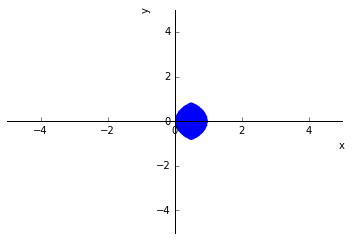
\includegraphics{images/optimization_01_1.png}
\caption{Page1}
\end{figure}

Note that the union is \textbf{not convex}: E.g. the union of
\(|| \mathbf{x}-\mathbf{0} ||^2 < 1\) and
\(|| \mathbf{x}- [2,0]^T < 1 ||^2\) is not convex.
